\documentclass[tikz,margin=2mm]{standalone}
\pagestyle{empty}

\usepackage{amsmath}
\usepackage{amssymb}
\usepackage{bm}
\usepackage{pifont}
\usetikzlibrary{positioning,calc, arrows,shapes}

\def\ci{\perp\!\!\!\!\!\perp}
\newcommand{\cmark}{\ding{51}}
\newcommand{\xmark}{\ding{55}}

\begin{document}
	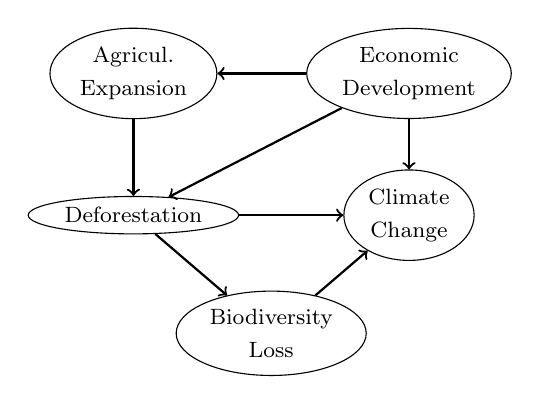
\begin{tikzpicture}
		\begin{scope}[scale=1]
		\tikzstyle{every node}=[draw, ellipse, align=center, inner sep=2pt]
			\node (D) at (0, 0) {\footnotesize{Deforestation}};
			\node (CC) at (3.5, 0) {\footnotesize Climate \\ \footnotesize Change};
			\node (BL) at (1.75, -1.5) {\footnotesize Biodiversity \\ \footnotesize Loss};
			\node (ED) at (3.5, 1.8) {\footnotesize Economic \\ \footnotesize Development};
			\node (AE) at (0, 1.8) {\footnotesize Agricul. \\ \footnotesize Expansion};
			
			\draw[->, thick]  (D) -- (CC);
			\draw[->, thick]  (D) -- (BL);
			\draw[->, thick]  (BL) -- (CC);
			\draw[->, thick]  (ED) -- (D);
			\draw[->, thick]  (ED) -- (AE);
			\draw[->, thick]  (AE) -- (D);
			\draw[->, thick]  (ED) -- (CC);
		\end{scope}

	\end{tikzpicture}

	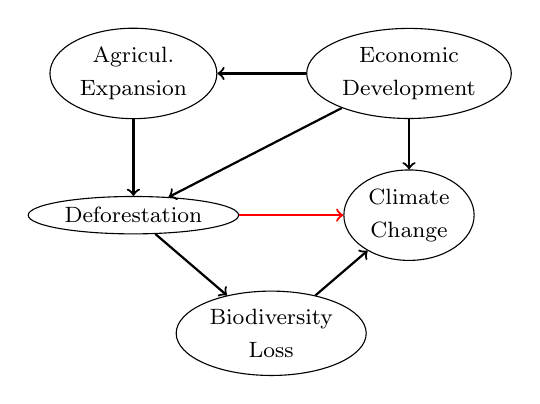
\begin{tikzpicture}
		\begin{scope}[scale=1]
		\tikzstyle{every node}=[draw, ellipse, align=center, inner sep=2pt]
			\node (D) at (0, 0) {\footnotesize{Deforestation}};
			\node (CC) at (3.5, 0) {\footnotesize Climate \\ \footnotesize Change};
			\node (BL) at (1.75, -1.5) {\footnotesize Biodiversity \\ \footnotesize Loss};
			\node (ED) at (3.5, 1.8) {\footnotesize Economic \\ \footnotesize Development};
			\node (AE) at (0, 1.8) {\footnotesize Agricul. \\ \footnotesize Expansion};
			
			\draw[->, thick, red]  (D) -- (CC);
			\draw[->, thick]  (D) -- (BL);
			\draw[->, thick]  (BL) -- (CC);
			\draw[->, thick]  (ED) -- (D);
			\draw[->, thick]  (ED) -- (AE);
			\draw[->, thick]  (AE) -- (D);
			\draw[->, thick]  (ED) -- (CC);
		\end{scope}
	\end{tikzpicture}

	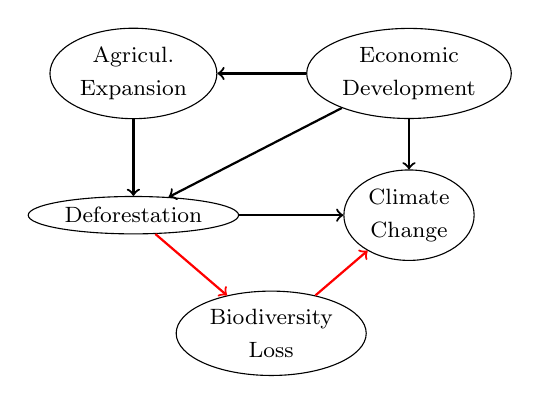
\begin{tikzpicture}
		\begin{scope}[scale=1]
		\tikzstyle{every node}=[draw, ellipse, align=center, inner sep=2pt]
			\node (D) at (0, 0) {\footnotesize{Deforestation}};
			\node (CC) at (3.5, 0) {\footnotesize Climate \\ \footnotesize Change};
			\node (BL) at (1.75, -1.5) {\footnotesize Biodiversity \\ \footnotesize Loss};
			\node (ED) at (3.5, 1.8) {\footnotesize Economic \\ \footnotesize Development};
			\node (AE) at (0, 1.8) {\footnotesize Agricul. \\ \footnotesize Expansion};
			
			\draw[->, thick]  (D) -- (CC);
			\draw[->, thick, red]  (D) -- (BL);
			\draw[->, thick, red]  (BL) -- (CC);
			\draw[->, thick]  (ED) -- (D);
			\draw[->, thick]  (ED) -- (AE);
			\draw[->, thick]  (AE) -- (D);
			\draw[->, thick]  (ED) -- (CC);
		\end{scope}
	\end{tikzpicture}

	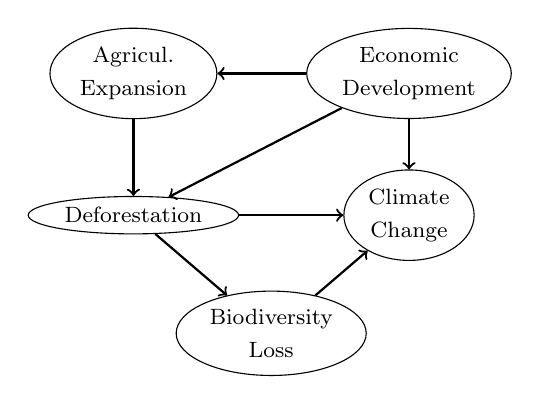
\begin{tikzpicture}
		\begin{scope}[scale=1]
		\tikzstyle{every node}=[draw, ellipse, align=center, inner sep=2pt]
			\node (D) at (0, 0) {\footnotesize{Deforestation}};
			\node (CC) at (3.5, 0) {\footnotesize Climate \\ \footnotesize Change};
			\node (BL) at (1.75, -1.5) {\footnotesize Biodiversity \\ \footnotesize Loss};
			\node (ED) at (3.5, 1.8) {\footnotesize Economic \\ \footnotesize Development};
			\node (AE) at (0, 1.8) {\footnotesize Agricul. \\ \footnotesize Expansion};
			
			\draw[->, thick]  (D) -- (CC);
			\draw[->, thick]  (D) -- (BL);
			\draw[->, thick]  (BL) -- (CC);
			\draw[->, thick]  (ED) -- (D);
			\draw[->, thick]  (ED) -- (AE);
			\draw[->, thick]  (AE) -- (D);
			\draw[->, thick]  (ED) -- (CC);
		\end{scope}
	\end{tikzpicture}

	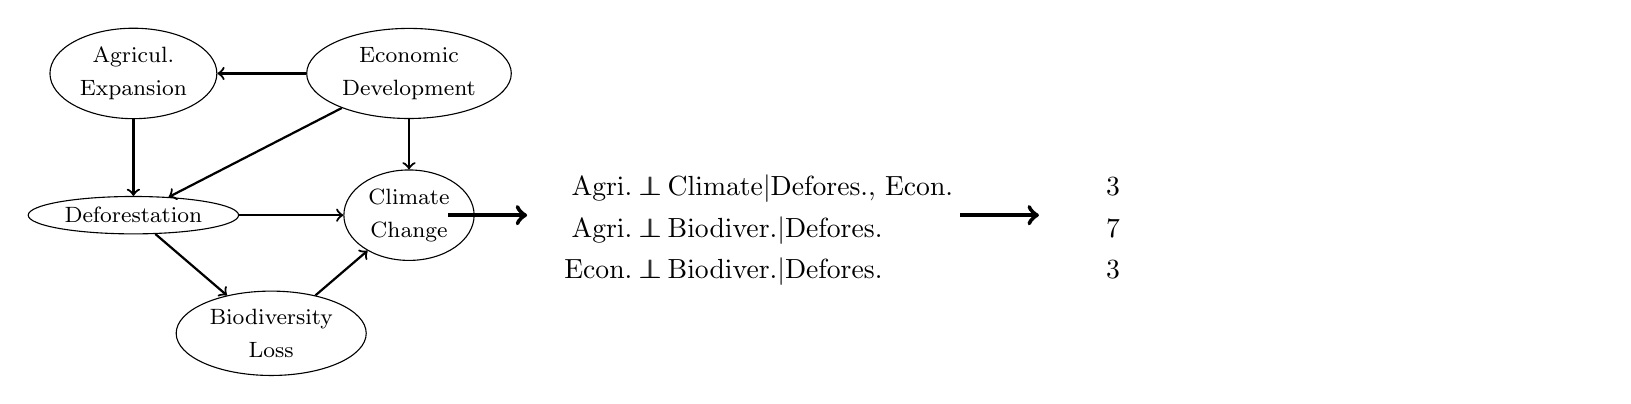
\begin{tikzpicture}
		\begin{scope}[scale=1]
		\tikzstyle{every node}=[draw, ellipse, align=center, inner sep=2pt]
			\node (D) at (0, 0) {\footnotesize{Deforestation}};
			\node (CC) at (3.5, 0) {\footnotesize Climate \\ \footnotesize Change};
			\node (BL) at (1.75, -1.5) {\footnotesize Biodiversity \\ \footnotesize Loss};
			\node (ED) at (3.5, 1.8) {\footnotesize Economic \\ \footnotesize Development};
			\node (AE) at (0, 1.8) {\footnotesize Agricul. \\ \footnotesize Expansion};
			
			\draw[->, thick]  (D) -- (CC);
			\draw[->, thick]  (D) -- (BL);
			\draw[->, thick]  (BL) -- (CC);
			\draw[->, thick]  (ED) -- (D);
			\draw[->, thick]  (ED) -- (AE);
			\draw[->, thick]  (AE) -- (D);
			\draw[->, thick]  (ED) -- (CC);
		\end{scope}
		\draw[ultra thick, ->] (4,0) -- (5,0);
		\node[rectangle, align=center, inner sep=1pt] at (8, 0) {
			\begin{minipage}{\textwidth}
				\begin{equation*}
					\begin{split}
						\textrm{Agri.} &\ci \textrm{Climate} \rvert \textrm{Defores., Econ.} \\
						\textrm{Agri.} &\ci \textrm{Biodiver.} \rvert \textrm{Defores.} \\
						\textrm{Econ.} &\ci \textrm{Biodiver.} \rvert \textrm{Defores.} \\
					\end{split}
				\end{equation*}
			\end{minipage}
		};
		\draw[ultra thick, ->] (10.5, 0) -- (11.5, 0);
		\node[rectangle, align=center, inner sep=1pt] at (12.5, 0){
				\begin{minipage}{\textwidth}
					\begin{equation*}
						\begin{split}
							& \cmark \\
							& \xmark \\
							& \cmark \\
						\end{split}
					\end{equation*}
				\end{minipage}
			};
	\end{tikzpicture}

	% \begin{tikzpicture}
	% 	\begin{scope}
	% 		\node[rectangle, align=center, inner sep=1pt] at (0, 0) {Data};
	% 	\end{scope}
	% 	\begin{scope}
	% 	\node[rectangle, align=center, inner sep=1pt] at (4, 0) {
	% 		\begin{minipage}{\textwidth}
	% 			\begin{equation*}
	% 				\begin{split}
	% 					\textrm{Age} &\ci \textrm{Incm} \rvert \textrm{Edct, Hrpw, Sex} \\
	% 					\textrm{Age} &\ci \textrm{Occp} \rvert \textrm{Edct, Sex} \\
	% 					\textrm{Age} &\ci \textrm{Sex} \\
	% 					\textrm{Hrpw} &\ci \textrm{Occp} \rvert \textrm{Edct, Sex} \\
	% 				\end{split}
	% 			\end{equation*}
	% 		\end{minipage}
	% 	\end{scope}
	% \end{tikzpicture}

\end{document}
